\newpage
\subsection{Aufbau}


Barth schreibt über Nagios: \begin{quote}"`Die große Stärke von Nagios - auch im Vergleich zu anderen Netzwerküberwachungstools - liegt in seinem modularen Aufbau: Der Nagios-Kern enthält keinen einzigen Test, stattdessen verwendet er für Service- und Host-Checks externe Programme, die als \textit{Plugins} bezeichnet werden."'
\begin{flushright}\cite{Barth08} S. 25\end{flushright}\end{quote} 

Dieser "`Kern"' beinhaltet das komplette Benachrichtigungssystem mit Kontaktadressen und Benachrichtigungsvorgaben (Zeit, Art, zusätzliche Kriterien), die Hosts- und Servicedefinitionen inklusive deren Gruppierungen und schließlich das Webinterface.

Die eigentlichen Checks in Form der selbständigen Plugins sind abgekapselt von diesem Kern, siehe Abbildung \ref{aktivechecks}.

\begin{figure}[ht]
	\centering
	   \fbox{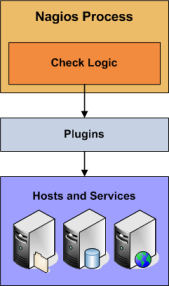
\includegraphics[scale=0.73]{bilder/activechecks.png}}
		\caption[Plugins als separate Komponente]{Plugins als separate Komponente\protect\footnote}
		\label{aktivechecks}
\end{figure} 
\footnotetext{Quelle: \url{http://nagios.sourceforge.net/docs/3_0/images/activechecks.png}}

Damit Nagios die gewünschten Server überwachen kann, müssen sie der Anwendung zuerst bekannt gemacht werden.
Dies wird über das Anlegen einer Konfigurationsdatei mit einem Host-Objekt erreicht.
Dabei richtet sich die Definition des Host-Objektes nach dem Schema, welches für alle Objektdefinitionen (Services, Kontakt, Gruppen, Kommandos etc.) gilt:

\begin{lstlisting}[captionpos=b, caption=Nagiosschema für Objektdefinitionen, label=schmeaobj, breaklines = false]
define object-type {
	parameter value
	parameter value ...		}
\end{lstlisting}


Eine gültige Host-Definition muss mindestens folgende Elemente besitzten:

\begin{lstlisting}[captionpos=b, caption=Definition eines Hostobjektes, label=hostobj, breaklines = true, language=sh]
define host{
	host_name		example.kit.edu #Referenzname des Servers
	alias			Oracle UCM Server #Weitere Bezeichnung
	address			example.kit.edu #FQDN des Rechners
	max_check_attempts	4 #Anzahl der Checks zum Wechsel von Soft- zu Hard-State
	check_period		24x7 #Zeitraum der aktiven Checks
	contact_groups		UCM-admins #Zu alarmierende Benutzergruppe
	notification_interval	120 #Minuten bis Alarmierung wiederholt wird
	notification_period	24x7 #Zeitraum der Benachrichtigungen
}
\end{lstlisting}

In der Praxis werden öfters verwendete Attribute wie die Kontaktgruppe oder der Zeitraum für die aktiven Checks durch Verwendung eines übergeordneten Host-Objektes nach unten vererbt.
Dadurch müssen nur noch die spezifischen Informationen des Servers eingetragen werden.
%und der Name des übergeordneten Host-Objektes
\begin{lstlisting}[captionpos=b, caption=Verkürzte Definition eines Hostobjektes, label=vhostobj, breaklines = true, language=sh]
define host {
        use             windows-server #Oberklasse dieses Host-Objektes
        host_name       example.kit.edu
        alias           Oracle UCM Server
        address         example.kit.edu		}
\end{lstlisting}

Mit dieser Hostdefinition wird der Rechner im Webinterface von Nagios bereits angezeigt:

\begin{figure}[ht]
	\centering
	   \fbox{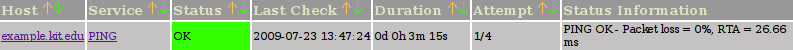
\includegraphics[width=0.85\textwidth]{bilder/example-ping.png}}
		\caption{Anzeige des Servers im Webinterface von Nagios}
		\label{check-swap}
\end{figure}

Damit wird die Erreichbarkeit über das Netzwerk mit einem Ping getestet.
%Umfangreichere / Komplexere / Weitergehende / 
Um weite Informationen zu erhalten, müssen die gewünschten Plugins explizit aus dem Nagios-Repertoire dem zu überwachendem Computer mit einem ähnlichen Schema zugeteilt werden.
Eine beispielhafte Servicedefinition für die Überwachung des Webservers auf dem Host \textit{example.kit.edu} wird in Codelisting \ref{servdef} gezeigt.

\begin{lstlisting}[captionpos=b, caption=Verkürzte Definition eines Hostobjektes, label=servdef, breaklines = true, language=sh]
define service{
        use		generic-service #Oberklasse dieses Service-Objektes
        host_name		example.kit.edu
        service_description     HTTP Server #Bezeichnung des Checks
        check_command		check_http #Angabe des Nagios-Plugins
        }
\end{lstlisting}

Die Plugins werden durch die Servicedefinitionen mit den jeweiligen Hosts verbunden und durch das Attribut \textit{check\_command} mit ggf. veränderten Parametern durch Nagios aufgerufen.
Nagios wird in einem modifizierbarem Zeitintervall alle vom Benutzer definierten Host- und Servicechecks überprüfen und die Ergebnisse der entsprechenden Plugins auswerten.
\paragraph{Nagios-Plugins und Ausgabe}
Weiterhin beschreibt Barth die Plugins folgendermaßen:
\begin{quote}"`Jedes Plugin, das bei Host- und Service-Checks zum Einsatz kommt, ist ein eigenes, selbständiges Programm, das sich auch unabhängig von Nagios benutzen lässt."' \begin{flushright}\cite{Barth08} S. 105\end{flushright}\end{quote} 
Daher lassen sich die Parameter eines Plugins in der Kommandozeile überprüfen:

\begin{figure}[ht]
	\centering
	   \fbox{
\includegraphics[width=0.7\textwidth]{bilder/check-swap-white.png}}
		\caption{Beispielhafte manuelle Ausführung eines Servicechecks}
		\label{check-swap}
\end{figure}

Die Ausgabe des Plugins gibt den Zustand des Services an.
In diesem Fall wird kein Schwellwert überschritten, daher die Meldung \pictext{SWAP OK}.
Dieses Plugin liefert noch zusätzliche Performance-Informationen, die mit externen Programmen ausgewertet, gespeichert und visualisiert werden können.
Standardmäßig werden die Performanzdaten von der normalen Ausgabe mit einem \pictext{|} getrennt.
Jedoch können auch Werte aus der normalen Textausgabe für die Visualisierung verwendet werden, so dass in diesem Beispiel keine Berechnung des Prozentsatzes notwendig wäre.

Um den Service mit den angegebenen Schwellwerten in Abbildung \ref{check-swap} von Nagios überwachen zulassen, muss folgende Servicedefinition in die Konfigurationsdatei eingetragen werden:

\begin{lstlisting}[captionpos=b, caption=Beispielhafte Definition eines Servicechecks, label=servdef, breaklines = true, language=bash]
#Test des Swap-Speichers mit WARNING und CRITICAL Schwellwertparameter
define service{
 use	generic-service 
 host_name	example.kit.edu 	
 service_description	Swap Disk Space
 check_command	check_swap!-w 20% -c 10%
}
\end{lstlisting}

Die Plugins liefern dabei verschiedene Rückgabewerte:
%\setlength{\tabcolsep}{50pt}
\begin{table}[!htbp]
\centering

\begin{tabular}{l l p{7cm}}
%\hline
\textbf{Status} \hspace{2 mm} & \textbf{Bezeichnung} \hspace{3 mm} & \textbf{Beschreibung}\\
\hline
%\textit{features} & complete\tnote{1} & complete\tnote{1} \\
%\hline
0 & OK & Alles in Ordnung \\
%\hline
1 & WARNING & Die Warnschwelle wurde überschritten, die kritische Schwelle ist aber noch nicht erreicht.\\
%\hline
2 & CRITICAL & Entweder wurde die kritische Schwelle überschritten oder das Plugin hat den Test nach einem Timeout  abgebrochen. \\
%\hline
3 & UNKNOWN &  Innerhalb des Plugins trat ein Fehler auf (zum Beispiel weil falsche Parameter verwendet wurden)\\
%\hline
\end{tabular}
\caption[Rückgabewerte für Nagios-Plugins]{Rückgabewerte für Nagios-Plugins\protect\footnote} %\protect\footnote
%\end{twoparttable}
\end{table}
\footnotetext{Quelle: \cite{Barth08} S. 105f}

Anhand dieser Werte wertet Nagios gezielt den Status des jeweiligen Objektes (Host oder Service) aus.
\paragraph{Hard und Soft States}
Weiterhin gibt es weiche (\pictext{Soft States}) und harte Zustände (\pictext{Hard States}):

\begin{figure}[ht]
	\centering
	   \fbox{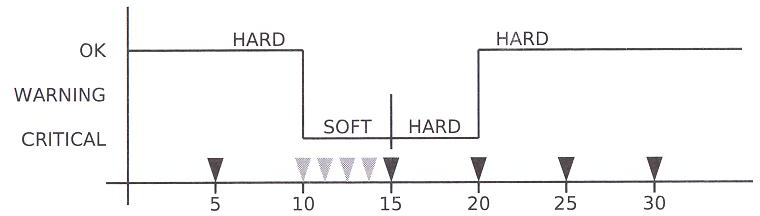
\includegraphics[width=0.85\textwidth]{bilder/hs-states.png}}
		\caption[Beispiel für den zeitlichen Verlauf durch vers. Zustände]{Beispiel für den zeitlichen Verlauf durch vers. Zustände\protect\footnote}
		\label{hs-states}
\end{figure}
\footnotetext{Quelle: \cite{Barth08} S. 95}
Ausgehend von einem \pictext{OK}-Zustand wird in diesem Beispiel jede fünf Minuten periodisch überprüft, ob sich der Status des überwachten Objektes verändert hat.                                                                                                                                                                                         Nach zehn Minuten wird eine Änderung des Zustandes durch das jeweilige Plugin gemeldet.
Hier im Beispiel wechselt der Zustand nach \pictext{CRITICAL}, zunächst allerdings als Soft State.
Daher wird durch Nagios noch keine Benachrichtigung versendet, da es sich um eine Falschmeldung, auch \textit{False Positive} genannt, handeln kann.
Aufgrund einer kurzfristigen hohen Auslastung des Netzwerkes oder um ein kurzzeitiges Problem, welches sich von alleine wieder normalisiert wie bspw. die Prozessorauslastung nach Beenden einer Anwendung.

Um False Positive-Meldungen zu verhindern, wird der im Soft State befindliche Service bzw. Host mit einer höheren Frequenz überprüft.
Sollten diese Überprüfungen den vorherigen Zustand bestätigen, verfestigt sich der aktuelle Zustand, man spricht nun von einem Hard State.
Erst in diesem Moment werden die entsprechenden Kontaktpersonen über den kritischen Zustand benachrichtigt.
Sollte sich der Zustand wieder in den Normalzustand begeben und dieser Zustandsübergang wird von dem Plugin festgestellt, wird dies an den Nagios-Server gemeldet.
Ein Übergang zu dem \pictext{OK}-Status wird sofort als Hard State festgesetzt und führt zur sofortigen Benachrichtigung durch Nagios.

\paragraph{Flapping}
Nagios besitzt eine spezielle Funktion um sich zu schnell ändernde Zustände automatisch zu erkennen und die Benachrichtigung von diesen Objekten zu unterbinden.
Das Verhalten dieser schnell wechselnde Zustände wird auch als \textit{Flapping} bezeichnet und deren Erkennung durch Nagios als \pictext{Flap Detection}.
Bei dieser Flap Detection speichert Nagios die letzten 20 Zustände und errechnet durch einen Algorithmus, welcher die aktuelleren Zustanden höher gewichtet, eine prozentuale Zustandsänderung.

Im folgenden Beispiel wurden sieben Zustandswechsel erfasst.
\begin{figure}[ht]
	\centering
	   \fbox{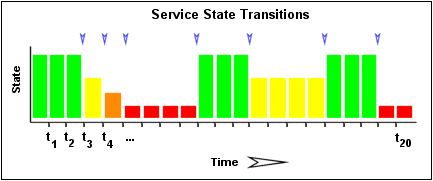
\includegraphics[width=0.85\textwidth]{bilder/statetransitions.png}}
		\caption[Verlauf von sich schnell wechselnden Zuständen]{Verlauf von sich schnell wechselnden Zuständen\protect\footnote}
		\label{hs-states}
\end{figure}
\footnotetext{Quelle: \url{http://nagios.sourceforge.net/docs/3\_0/images/statetransitions.png}}

Dadurch ergibt sich ein Wechselzustand von:

$$
\frac{7}{20} = 0,35 = 35\%
$$

Standardmäßig deklariert Nagios einen Host oder Service ab 25\% als Flapping und unterbindet die Benachrichtigung.

%Nagios supports optional detection of hosts and services that are "flapping". Flapping occurs when a service or host changes state too frequently, resulting in a storm of problem and recovery notifications. Flapping can be indicative of configuration problems (i.e. thresholds set too low), troublesome services, or real network problems. 

%\begin{itemize}
%\item Betroffene OSI Schichten auflisten und erklären
%\item Wie werden die Info von Nagios gesammelt und wie gespeichert -> FlapDetection
%\item FLapping \footnote{\url{http://nagios.sourceforge.net/docs/2\_0/flapping.html}}
%\item Benachrichtigung durch email oder sms sogar per Telefon geht usw.
%\item Hierarchie \url{http://nagios.sourceforge.net/docs/3_0/networkreachability.html}
%\end{itemize}